\documentclass[xcolor=dvipsnames]{beamer}
\usetheme{Boadilla}

\definecolor{HKARedPrim}{RGB}{215, 34, 5}
\definecolor{HFUGreenSec}{RGB}{0, 132, 77}
\definecolor{HFUGrey}{RGB}{218, 220, 220}
\definecolor{HFUAnthr}{RGB}{112, 113, 115}
\usecolortheme[named=HKARedPrim]{structure}
\setbeamertemplate{section in toc}[circle]
\setbeamertemplate{subsection in toc}[square]

\setbeamertemplate{frametitle}{\vspace{0.9em}\textbf{\insertframetitle}}

\usepackage[T1]{fontenc}
\usepackage[english]{babel}
\usepackage{graphicx}
\usepackage{eso-pic}
\usepackage{caption}
\usepackage{bytefield}

\usepackage{listings}
\lstdefinestyle{customc}{
	belowcaptionskip=1\baselineskip,
	breaklines=true,
	numbers=left,
	columns=flexible,
	xleftmargin=2em,
	xrightmargin=1em,
	firstnumber=1,
	numberfirstline,
	numberstyle=\tiny\sffamily,
	numbersep=6pt,
	basicstyle=\footnotesize\ttfamily,
	keywordstyle=\bfseries\color{green!40!black},
	commentstyle=\itshape\color{purple!40!black},
	identifierstyle=\color{blue},
	backgroundcolor=\color{gray!10!white},
}
\lstset{style=customc}
\lstset{captionpos=b}

\title[Seminararbeit]{\textbf{Seminararbeit}}
\subtitle{Dynamische Programmanalysen für nebenläufige Programme - Data Race Prediction mit TSan}
\author[Frank Ling]{
\includegraphics[trim={1230px 0 0 0}, clip, scale=0.1]{pics/HKA_Logo_Logoleiste_RGB.png}\\Frank Ling}
\date{June 13, 2023}
\setbeamertemplate{itemize item}{$\circ$}

\begin{document}
	
	\frame{\titlepage}
	
	\newcommand\AtPagemyUpperLeft[1]{\AtPageLowerLeft{%
			\put(\LenToUnit{0.6\paperwidth},\LenToUnit{0.86\paperheight}){#1}}}
	\AddToShipoutPictureFG{
		\AtPagemyUpperLeft{{
\includegraphics[scale=0.06]{pics/HKA_Logo_Logoleiste_RGB.png}}}
	}%
	
	\frame{
		\frametitle{Table of contents}
		\tableofcontents
	}
	
	\section{Introduction}
	\frame{
		\frametitle{Introduction}
		\begin{columns}
			\begin{column}{0.5\textwidth}
				\begin{itemize}[<+->]
					\item What are data races?
					\item Why fix data races?
					\item How to detect data races?
				\end{itemize}
			\end{column}
			\begin{column}{0.5\textwidth}
				\centering
				\begin{figure}
					\hspace{-2em}
					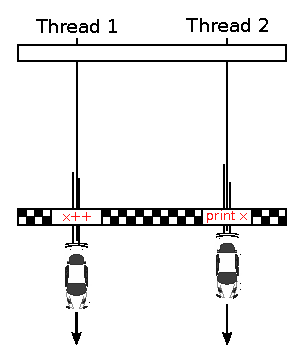
\includegraphics[scale=0.6]{pics/data-race.pdf}
					\caption*{\tiny Source: \url{https://programming.guide/go/data-races-explained.html}}
				\end{figure}
			\end{column}
		\end{columns}
	}

	\section{Background}
		\begin{frame}[fragile]
			\frametitle{Background}
			\begin{columns}
				\begin{column}{0.55\textwidth}<1->
				\begin{lstlisting}[caption={program exhibiting a data race},language=C++]
int x;
pthread_mutex_t y;

void *Thread1(void *x) {
	x++;
	pthread_mutex_lock(&y);
	pthread_mutex_unlock(&y);
	return NULL;
}

void *Thread2(void *x) {
	pthread_mutex_lock(&y);
	x--;
	pthread_mutex_unlock(&y);
	return NULL;
}
				\end{lstlisting}
				\end{column}
				\begin{column}{0.5\textwidth}<2->
					\begin{table}
						\begin{center}
							\begin{tabular}{ c c c}
								& 1\# & 2\# \\
								\hline
								1. & w(x) & \\
								2. & acq(y) & \\
								3. & rel(y) & \\
								4. & & acq(y) \\
								5. & & w(x) \\
								6. & & rel(y) \\
							\end{tabular}
						\caption{obtained trace}
						\label{trace1}
						\end{center}
					\end{table}
				\end{column}
			\end{columns}
			
		\end{frame}
	
	\frame{
		\begin{columns}
			\begin{column}{0.5\textwidth}<2->
				\Large\hspace{4em}Data race! \hspace{2em}$\Leftarrow$
			\end{column}
			\begin{column}{0.5\textwidth}<1->
				\begin{table}
					\begin{center}
						\begin{tabular}{ c c c}
							& 1\# & 2\# \\
							\hline
							4. & & acq(y) \\
							5. & & w(x) \\
							1. & w(x) & \\
							6. &  & rel(y) \\
							2. & acq(y) & \\
							3. & rel(y) & \\
						\end{tabular}
						\caption{Trace \ref{trace1} reordered}
						\label{trace2}
					\end{center}
				\end{table}
			\end{column}
		\end{columns}
		
	}
		
	
	\frame{
		\frametitle{Background}
			\begin{itemize}[<+->]
				\item Dynamic data race prediction
				\item Vector clocks
				\item Epochs
				\item Lamport's HB relation
			\end{itemize}
	}

	\frame{
		\frametitle{Lamport's HB relation}
		\begin{columns}[t]
			\begin{column}{0.4\textwidth}
				Program order condition
				\begin{itemize}
					\item For events $e$ and $f$ in same thread, if $e$ appears before $f$ in trace then $e<_{HB}f$
					\item $\text{inc}(V,j)$ applied after processing event in same thread
				\end{itemize}
			\end{column}
			\begin{column}{0.45\textwidth}
				Critical section
				\begin{itemize}
					\item For rel(y) in thread $i$ and acq(y) in thread $j$ if rel(y) appears beofre acq(y) then $\text{rel}(y)<_{HB}\text{acq}(y)$
					\item $\text{sync}(V_1, V_2)$ is applied after rel(y) in thread 
				\end{itemize}
			\end{column}
		\end{columns}
	}

	
	\section{FastTrack and TSan V2}
	\frame{
		\frametitle{FastTrack and TSan V2}
		\begin{columns}[t]
			\begin{column}{0.5\textwidth}
				FastTrack
				\begin{itemize}
					\item Lamport's HB relation
					\item epoch-based
					\item semi-adaptive
					\begin{itemize}
						\item dynamically sized epochs expensive
						\item initially epochs only
						\item read $\rightarrow$ VC, stays VC after (subsequent concurrent reads frequent)
						\item writes are epochs only (all writes are totally ordered)
					\end{itemize}
				\end{itemize}
			\end{column}
			\begin{column}{0.425\textwidth}
				ThreadSanitizer (TSan) V2
				\begin{itemize}
					\item slightly modified version of FastTrack
					\item shadow memory
				\end{itemize}
			\end{column}
		\end{columns}
	}

	\begin{frame}[fragile]
		\frametitle{Shadow memory}
		\begin{columns}[t]
			\begin{column}{0.5\textwidth}
				\begin{itemize}[<+->]
					\item Shadow word (64 bits)\\\vspace{0.5em}
					\begin{tabular}{| c | c |}
						\hline
						TID (Thread Id) & 16 bits \\
						\hline
						Scalar Clock & 42 bits \\
						\hline
						IsWrite & 1 bit \\
						\hline
						Access Size & 2 bits \\
						\hline
						Address Offset & 3 bits \\
						\hline
					\end{tabular}
					\vspace{1em}
					\item \textbf{N} shadows words\\ \hspace{3em}$\downarrow$\\ application word (memory location)
				\end{itemize}
			\end{column}
			\begin{column}{0.5\textwidth}
				\begin{itemize}[<+->]
					\item N is configurable (2, 4, 8) but default is 4 \\\hspace{5em}$\Downarrow$\\For every memory location 1 write and up to concurrent 3 reads are stored
					\item for every subsequent concurrent read a random read in shadow memory will be evicted
				\end{itemize}
			\end{column}
		\end{columns}
	\end{frame}
	
	\subsection{Limitations}
	\begin{frame}[fragile]
		\frametitle{Limitations}
		\begin{columns}
			\begin{column}{0.5\textwidth}
			\begin{itemize}
				\item Unsound due to epochs
			\end{itemize}
			\begin{lstlisting}[caption={program showing unordered writes}]
void thread1() {
	y := x+5;
}

void thread2() {
	if (y == 5)
		x := 10;
	else
		while(true);
}
			\end{lstlisting}	
			\end{column}
		\hspace{1em}
		\begin{column}{0.5\textwidth}
			\begin{table}
				\begin{center}
					\begin{tabular}{ c c c}
						& 1\# & 2\# \\
						\hline
						1. & r(x) & \\
						2. & w(y) & \\
						3. & & r(y) \\
						4. & & w(x) \\
					\end{tabular}
					\caption{Obtained trace}
				\end{center}
			\end{table}
		\end{column}
		\end{columns}
	\end{frame}
	
	\frame{
		\frametitle{Limitations}
		\begin{itemize}
			\item Incomplete due to:
			\begin{itemize}
				\item HB relation (see first example)
				\item shadow memory
			\end{itemize}
		\end{itemize}
	}

	
	\section{Conclusion}
	\frame{
		\frametitle{Conclusion}
		\begin{itemize}
			\item no race detection tool right now is entirely complete and sound
			\item FastTrack and TSan produce good results even though missing data races under certain circumstances
			\item they are reasonably efficient compared to other data race detection tools
		\end{itemize}
	}
	
\end{document}
